\documentclass[aspectratio=43,unicode,10pt]{beamer}
\usetheme{ttipresentation}

\usepackage{luatexja}
\usepackage{luatexja-fontspec}
\usepackage{graphicx}
\usepackage{calc}
\usepackage[overlay,absolute]{textpos}

\setlength{\TPHorizModule}{\textwidth}
\setlength{\TPVertModule}{\textheight}
\newlength\horizoffset
\setlength{\horizoffset}{1in+\hoffset+\oddsidemargin}
\newlength\vertoffset
\setlength{\vertoffset}{1in+\voffset+\topmargin+\headheight+\headsep}
\textblockorigin{\horizoffset}{\vertoffset}

\setmainjfont{ipagp.otf}
\beamertemplatenavigationsymbolsempty
\newcommand{\itemtitle}[1]{\textbf{#1}\\}
\newcommand{\fire}[1]{\textcolor{red}{\textbf{#1}}}
\newcommand{\freeze}[1]{\textcolor{blue}{\textbf{#1}}}
\newcommand{\then}{\textcolor{ttiblue}{\textbf{⇒}}\hspace{1ex}}
\newcommand{\up}{\textcolor{orange}{\textbf{◎}}\hspace{1ex}}


\title{文書・文間及びカテゴリ間の関係を\\考慮したレーティング予測}
\institute{知能数理研究室}
\author{12056 外山 洋太}
\date{\today}



\begin{document}

\begin{frame}
\titlepage
\end{frame}

\begin{frame}{研究背景}{}
  \begin{block}{多カテゴリにおける商品レビューのレーティング予測}
    \begin{itemize}
      \item カテゴリ:レーティングの付く各項目のこと
      \item \fire{文同士の位置関係}及び\fire{カテゴリ間の関係}が重要
    \end{itemize}
  \end{block}
  \begin{figure}
    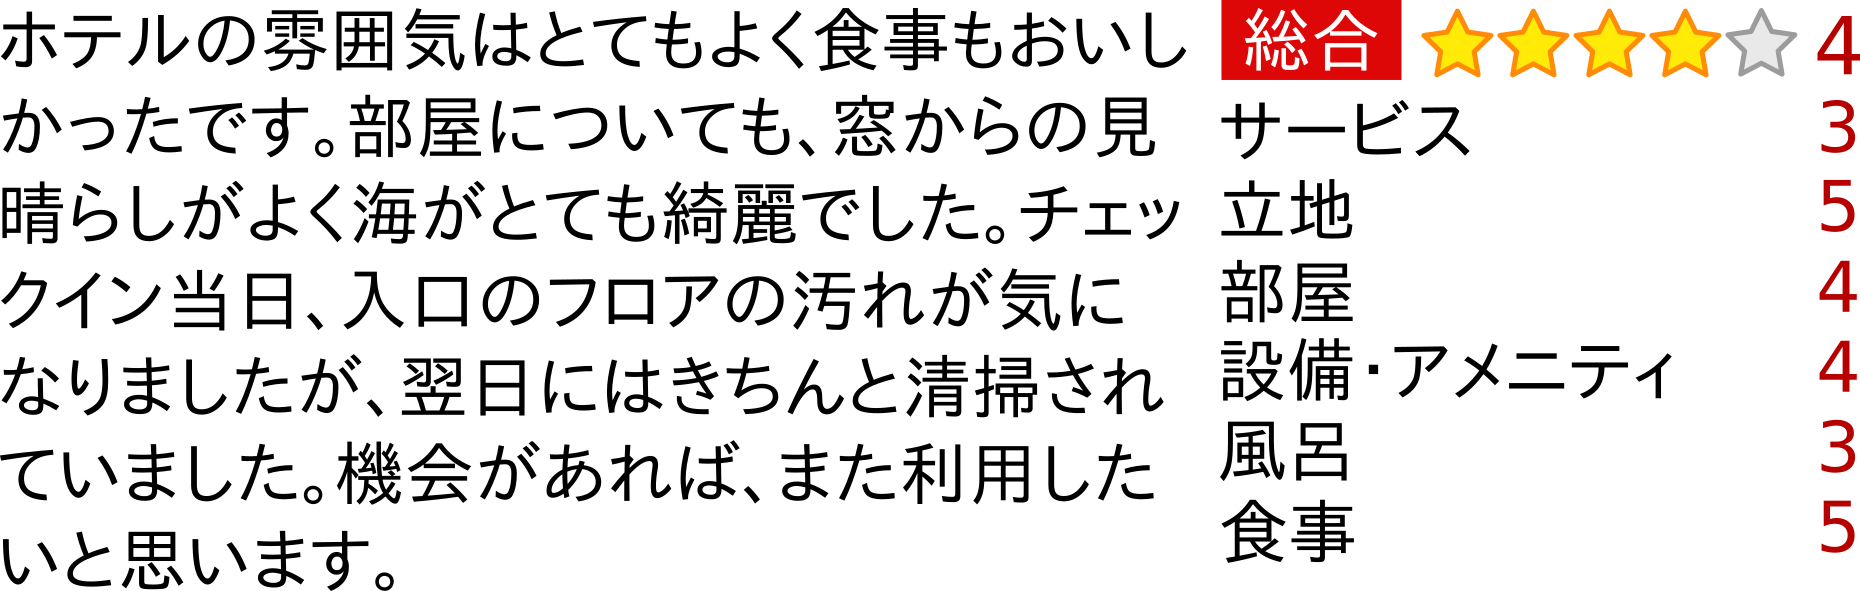
\includegraphics[width=0.9\linewidth]{fig/review.png}
  \end{figure}
\end{frame}

\begin{frame}{研究背景}{}
  \begin{block}{文同士の位置関係}
    \begin{figure}
      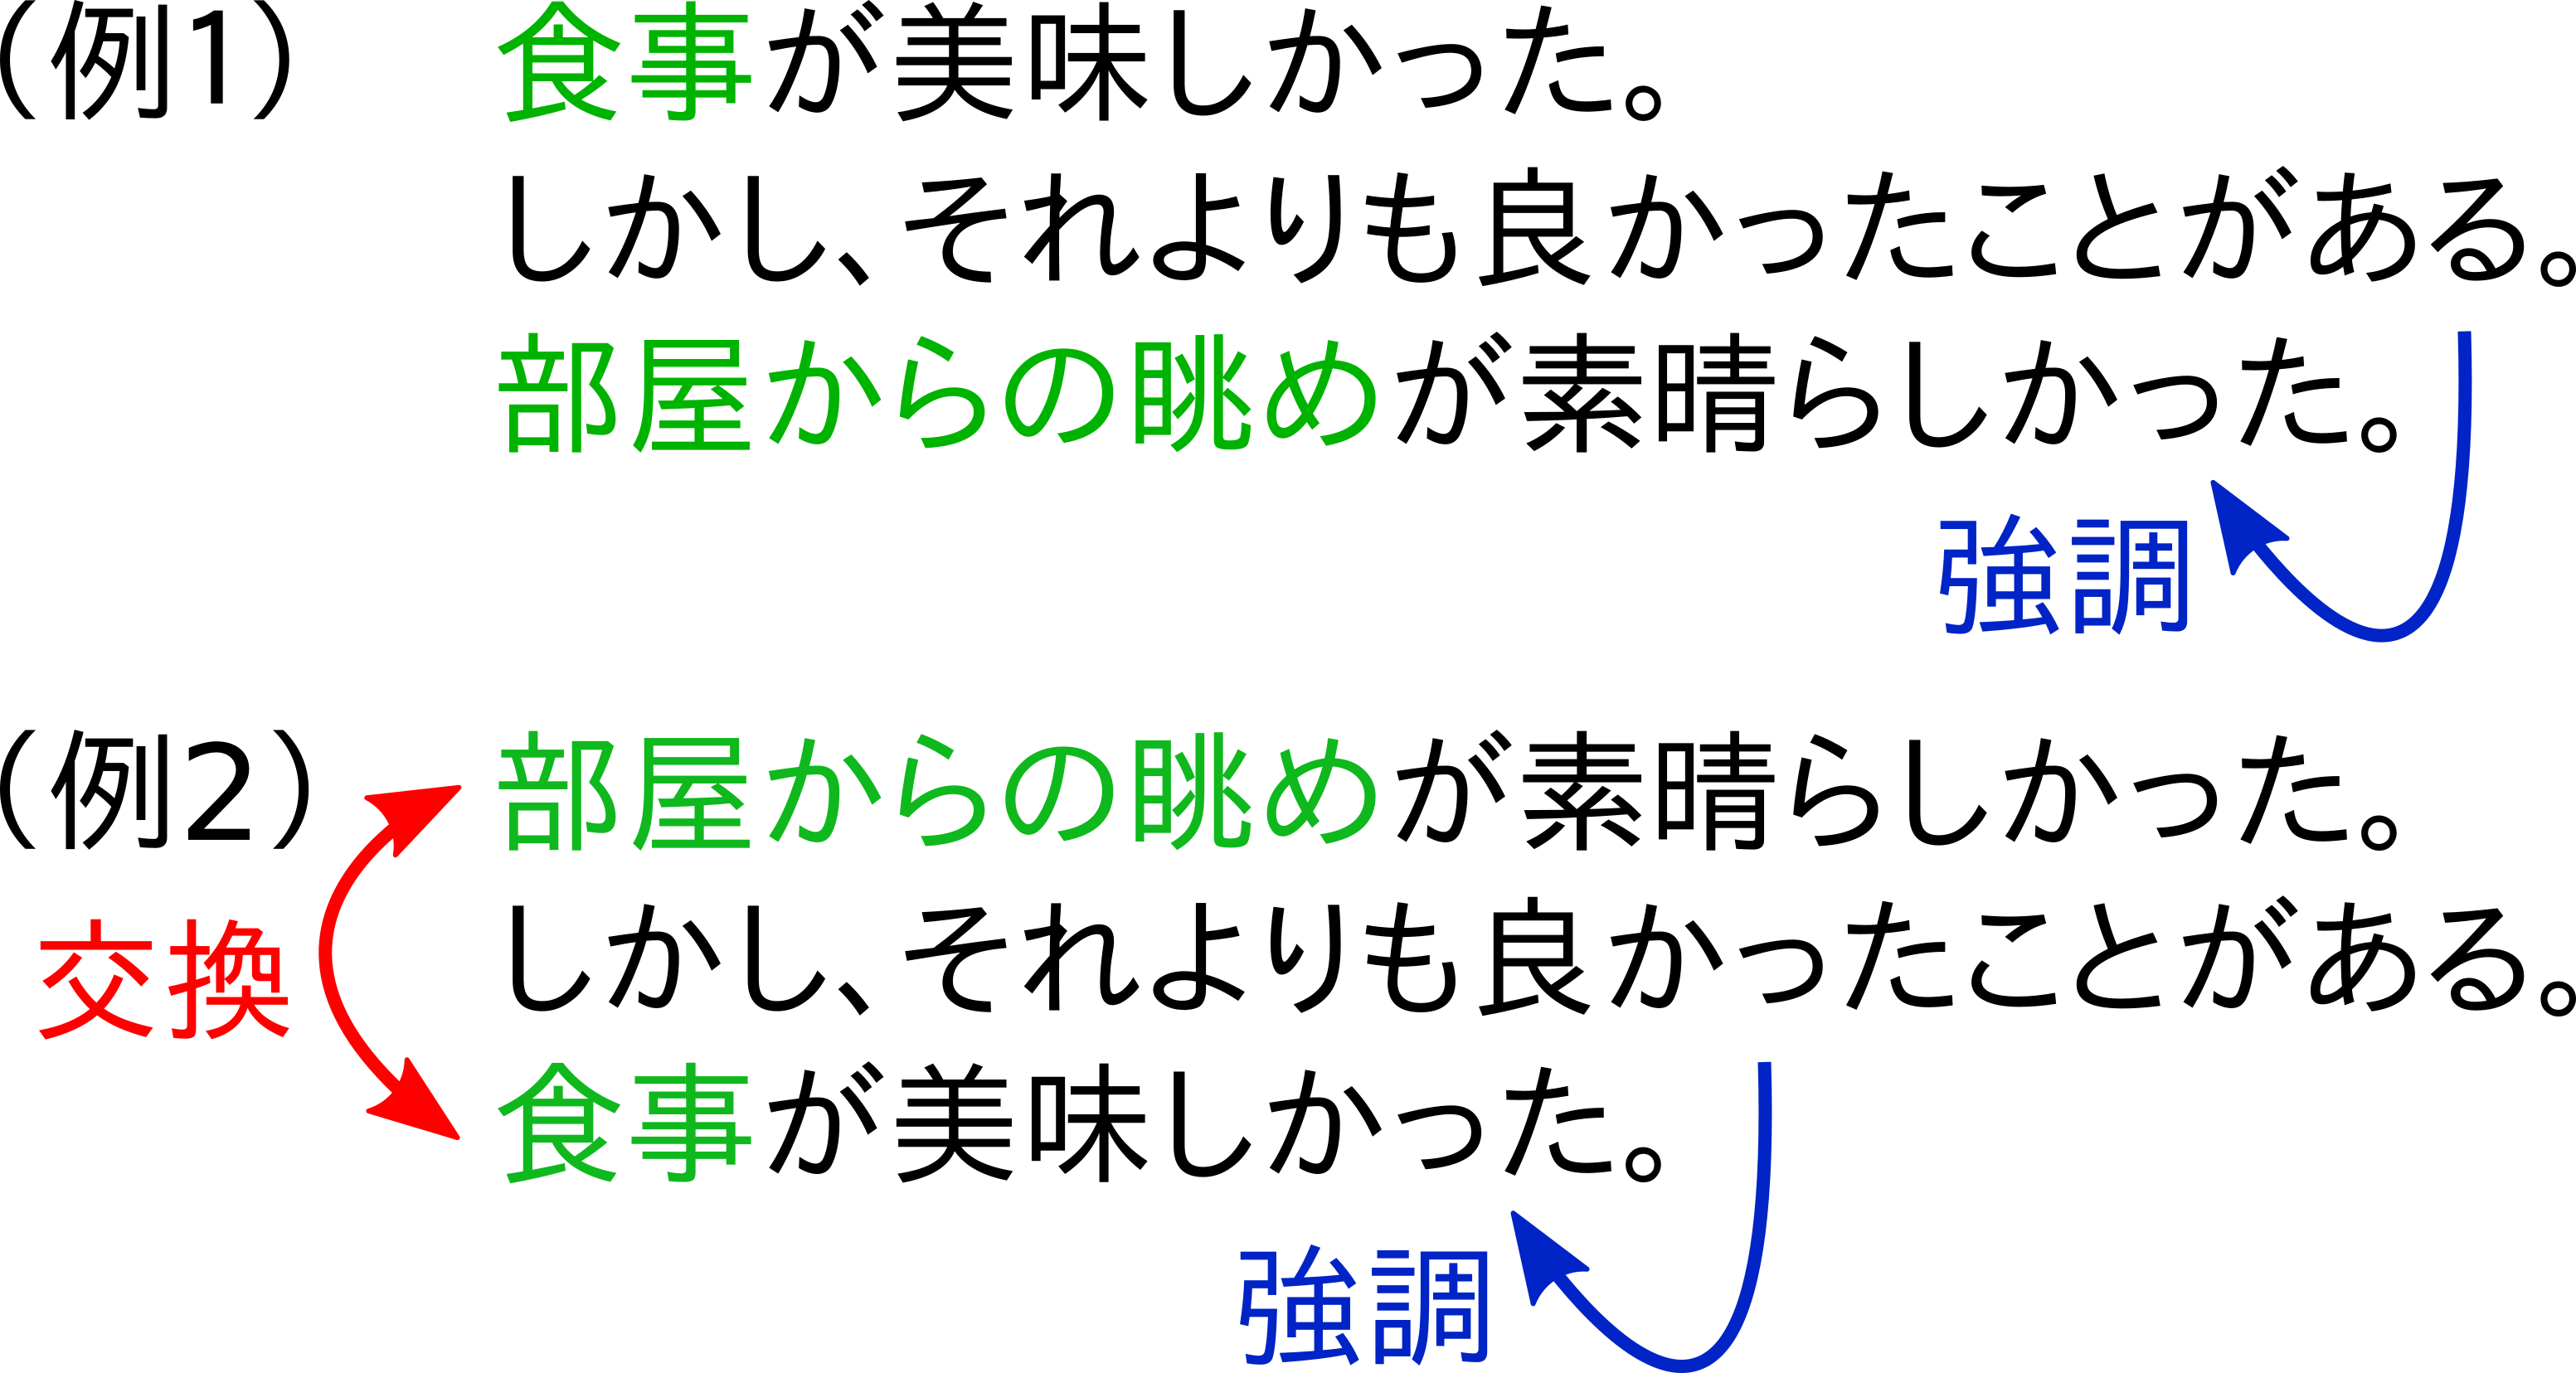
\includegraphics[width=0.8\linewidth]
                      {fig/relations_among_sentences.png}
    \end{figure}
  \end{block}
\end{frame}

\begin{frame}{研究背景}{}
  \begin{block}{カテゴリ間の関係}
    \begin{itemize}
      \item 食事\up \then サービス\up
      \item 設備・アメニティ\up \then サービス\up
    \end{itemize}
    \begin{figure}
      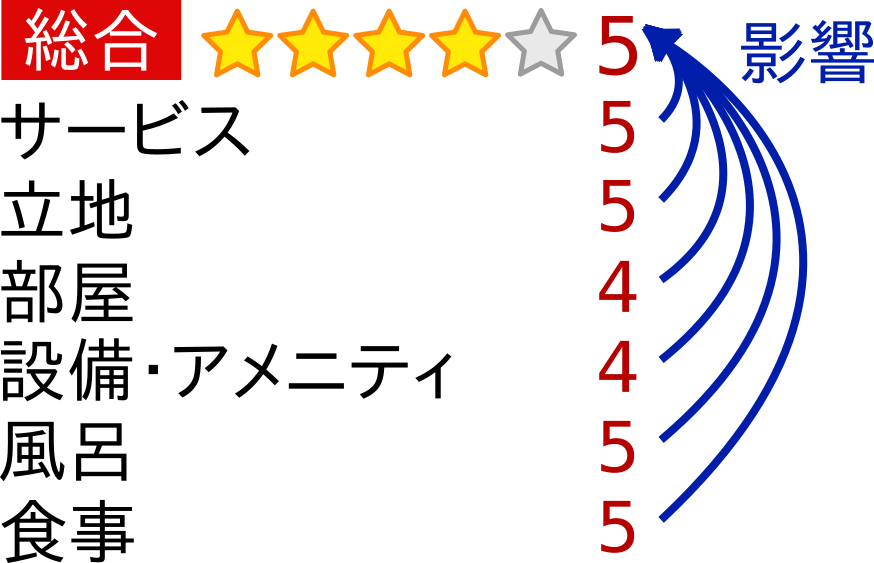
\includegraphics[width=0.5\linewidth]
                      {fig/relations_among_rating_categories.png}
    \end{figure}
  \end{block}
\end{frame}

\begin{frame}{関連研究}{}
  \begin{block}{隠れ状態を用いたホテルレビューのレーティング予測}
    \begin{itemize}
      \item 文毎のレーティングからレビュー全体のレーティングを予測
      \item カテゴリ間の繋がりを\freeze{手調整で変化}させて考慮
    \end{itemize}
  \end{block}
  \begin{block}{パラグラフベクトル}{}
    \begin{itemize}
      \item 文や文書を、その意味を表す実数ベクトルに変換する手法
      \item \fire{評判分類において優れる}
    \end{itemize}
  \end{block}
  \begin{block}{ニューラルネットワーク}{}
    \begin{itemize}
      \item 神経回路を模した機械学習手法
      %\item 分類問題に適用可能
      \item \fire{入力の要素間の複雑な関係}を考慮
    \end{itemize}
  \end{block}
\end{frame}

\begin{frame}{提案手法}{}
  \begin{block}{レーティング予測の流れ}
    %\begin{enumerate}
    %  \item パラグラフベクトルにより各レビューとその中の文のベクトルを生成
    %  \item 文ベクトルをレビュー毎に圧縮
    %  \item ニューラルネットワークによりレーティングを予測
    %\end{enumerate}
    \begin{figure}
      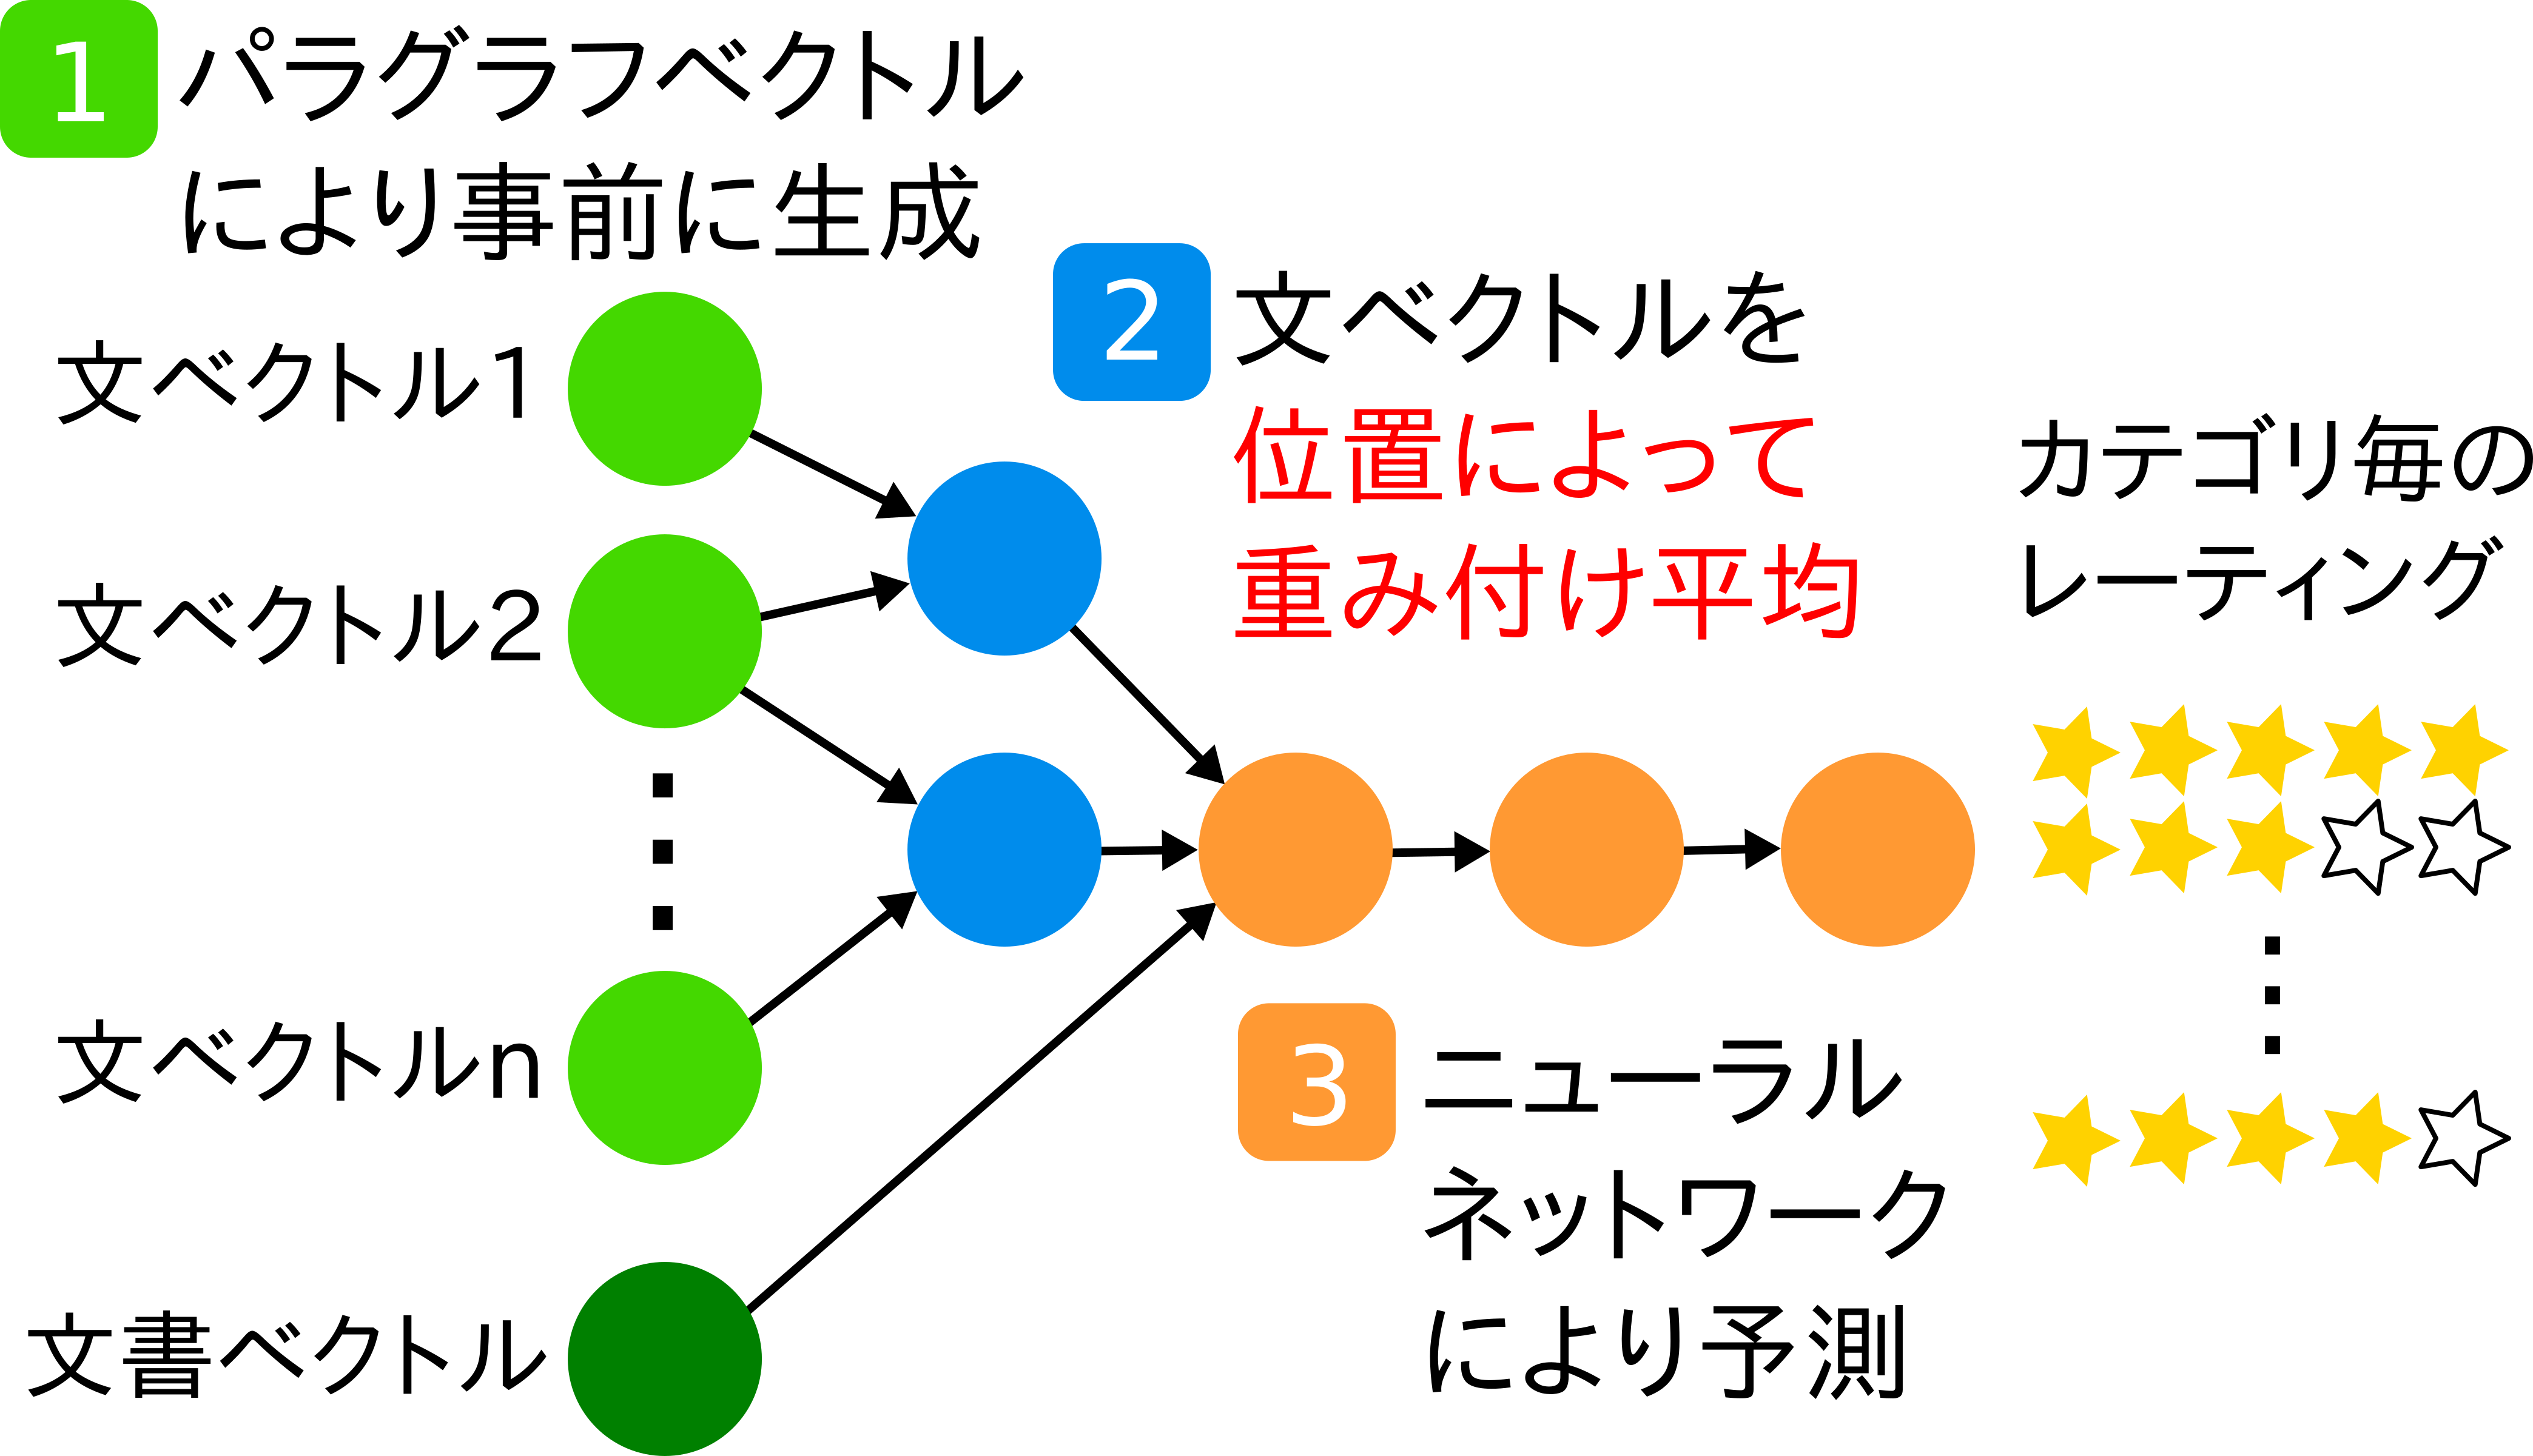
\includegraphics[width=0.9\linewidth]
                      {fig/model_with_detailed_processes.png}
    \end{figure}
  \end{block}
\end{frame}

\begin{frame}{実験及び結果}{}
  \begin{block}{実験設定}
    \begin{itemize}
      \item 7カテゴリにおける0〜5点のレーティング予測の正答率を測定
      \item データセット:楽天トラベルにおけるレビュー約330,000件
    \end{itemize}
  \end{block}
  \begin{block}{結果}
    \begin{columns}[onlytextwidth,t]
      \begin{column}{0.6\linewidth}
        \begin{itemize}
          \item 提案手法が従来手法より\fire{高い正答率}を示した
          %\item \fire{文の並び}が予測のために重要
          %\item 文書ベクトルと文ベクトルを同時に用いることが有効
        \end{itemize}
      \end{column}
      \begin{column}{0.4\linewidth}
        \begin{table}
          \centering
          \begin{tabular}{l | r} \label{tab:Accuracies}
            手法 & 正答率 \\
            \hline
            従来手法 & 0.4832 \\
            提案手法 & \fire{0.5030} \\
          \end{tabular}
        \end{table}
      \end{column}
    \end{columns}
  \end{block}
\end{frame}

\end{document}
